%----------------------------------------------------------------------------------------
%	SOLUTION 2
%----------------------------------------------------------------------------------------
\subsection*{Problem 2}
The dynamic system in this problem is given by,
\begin{align*}
	\dot{x} &= w\\
	\mathbb{E}[w] &= 0\\
	\mathbb{E}[w(t)w(\tau)] &= Q_c\delta(t-\tau)\\
	Q_c &= 1.
\end{align*}
%----------------------------------------------------------------------------------------
%	SOLUTION 2.a
%----------------------------------------------------------------------------------------
\paragraph{2.a} The dynamic system equation can be written as:
\begin{align*}
	\dot{x} &= 0x + 0u + w.
\end{align*}
Therefore, $A=0$ and $B=0$.
%----------------------------------------------------------------------------------------
%	SOLUTION 2.b
%----------------------------------------------------------------------------------------
\paragraph{2.b} $F$ and $G$ matrices of the discretized system can be derived as:
\begin{align*}
	F &= e^{AT}\\
	&= 1,
\end{align*}
where $T$ is the sampling interval equal to $1$ sec. Also,
\begin{align*}
	G &= e^{AT}\int_{0}^{T}e^{-A\alpha}\text{d}\alpha B\\
	&= 0.
\end{align*}
%----------------------------------------------------------------------------------------
%	SOLUTION 2.c
%----------------------------------------------------------------------------------------
\paragraph{2.c}The covariance of discrete process noise is:
\begin{align*}
	Q &= \int_{t_{k-1}}^{t_k}\int_{t_{k-1}}^{t_k}e^{A(t_k-\tau)}\mathbb{E}[w(\tau)w(\alpha)]e^{A^T(t_k-\alpha)}\text{d}\tau\text{d}\alpha\\
	&= \int_{t_{k-1}}^{t_k}\int_{t_{k-1}}^{t_k} Q_c \delta(\tau-\alpha)\text{d}\tau\text{d}\alpha\\
	&= \int_{t_{k-1}}^{t_k}Q_c\text{d}\tau\\
	&= Q_c(t_k-t_{k-1})\\
	&= Q_cT\\
	&= T\\
	&= 1.
\end{align*}
%----------------------------------------------------------------------------------------
%	SOLUTION 2.d
%----------------------------------------------------------------------------------------
\paragraph{2.d}The plot from the Monte-Carlo simulation is shown in Fig.~\ref{fig:q2_d}.
\begin{figure}[h]
	\centering
	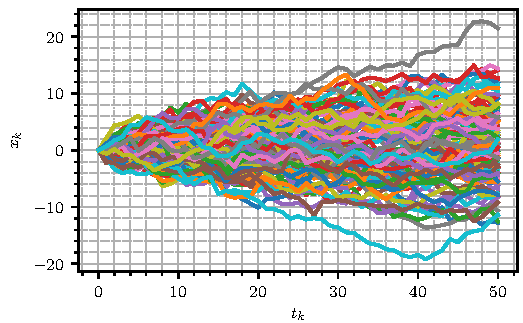
\includegraphics[scale=1.0,trim={0cm 0cm 0cm 0cm},clip]{./code/generatedPlots/q2_d.pdf}
	\caption{Q2.d: Monte-Carlo simulation of the dynamic process}
	\label{fig:q2_d}
\end{figure}
Ensemble standard deviation at $t_k=5,25$ and $50$ are $2.044, 4.99$ and $6.49$ respectively.
%----------------------------------------------------------------------------------------
%	SOLUTION 2.e
%----------------------------------------------------------------------------------------
\paragraph{2.e}The plot from the Monte-Carlo simulation is shown in Fig.~\ref{fig:q2_e}.
\begin{figure}[h]
	\centering
	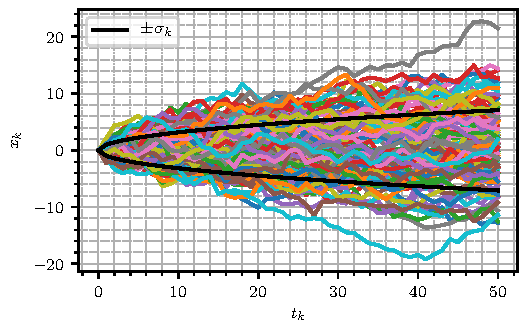
\includegraphics[scale=1.0,trim={0cm 0cm 0cm 0cm},clip]{./code/generatedPlots/q2_e.pdf}
	\caption{Q2.e: Monte-Carlo simulation along with plot from covariance analysis}
	\label{fig:q2_e}
\end{figure}
Values of $\sigma$ at $t_k=5$ and $10$ are $2.23$ and $3.16$ respectively.
%----------------------------------------------------------------------------------------
%	SOLUTION 2.f
%----------------------------------------------------------------------------------------
\paragraph{2.f}If I do not have any historical state measurements in hand, I would go for covariance analysis because it gives the theoretical state estimate standard deviation while to prove that Monte-Carlo simulation gives an accurate prediction of covariance, I need to run the simulation for many time, ideally infinite times. Usually, we go for Monte-Carlo where it is not possible to calculate the quantity theoretically. However, If I have historical state measurements in hand, I can check for any outliers or modeling error by doing Monte-Carlo analysis and compare that with the historical measurements.